\documentclass[11pt]{article}
\usepackage[margin=1in]{geometry}
\usepackage{graphicx,amsmath,amssymb,microtype}
\usepackage[dvipsnames]{xcolor}
\usepackage[colorlinks=true,allcolors=blue!55!black]{hyperref}
\usepackage{tcolorbox}
\graphicspath{{../results/figures/}}
\definecolor{navy}{HTML}{0b1f3a}\definecolor{teal}{HTML}{1f9e89}\definecolor{amber}{HTML}{f0a202}
\newtcolorbox{key}[1][]{colback=teal!8,colframe=teal,boxrule=0.8pt,arc=3pt,left=6pt,right=6pt,top=4pt,bottom=4pt,#1}
\newtcolorbox{ana}[1][]{colback=amber!8,colframe=amber!80!black,boxrule=0.7pt,arc=3pt,left=6pt,right=6pt,top=4pt,bottom=4pt,#1}
\newcommand{\term}[1]{\textbf{\color{navy}#1}}
\renewcommand{\familydefault}{\sfdefault}
\title{\vspace{-2em}\textbf{\color{navy}\Large Reading the Dark Matter of the Genome}\\[2mm]
\large A ground-up guide to how POLARIS predicts whether a non-coding DNA variant causes disease}
\author{}\date{\vspace{-3em}}
\begin{document}\maketitle

\noindent\textit{This guide assumes no biology or statistics background. Each idea is built from the
one before it. By the end you will understand a research-grade pipeline for one of the hardest open
problems in human genetics --- and why every step is necessary.}

\section{Start here: DNA, genes, and ``variants''}
Your \term{genome} is a 3-billion-letter instruction book written in a 4-letter alphabet: A, C, G, T.
It is copied into nearly every cell. Stretches of it called \term{genes} are recipes for \term{proteins},
the molecular machines that do most of the work in a cell.

People differ from one another at millions of single positions in this book. A position where the letter
commonly differs between people is a \term{variant} (for example, most people have a C at some spot, but
some have a T). Most variants are harmless. A few change how the body works and can raise the risk of
disease. \emph{The central question of this project is: given a variant, can we tell whether---and how---it
contributes to a disease?}

\begin{ana}
\textbf{Analogy.} Think of the genome as a cookbook. Genes are recipes. A variant is a single changed
character. Some changes are typos in a word you never read (harmless); some change ``1 cup sugar'' to
``2 cups'' (consequential). We want to find the consequential ones and explain \emph{why} they matter.
\end{ana}

\section{The twist: most disease variants are \emph{not} in recipes}
Only about 2\% of the genome is genes (recipes). The other 98\% was once dismissed as ``junk,'' but much
of it is \term{regulatory}: it controls \emph{when}, \emph{where}, and \emph{how much} each gene is used.
Think of \term{enhancers} as dimmer switches wired to specific genes.

Strikingly, about \textbf{90\%} of variants linked to common diseases lie in this non-coding,
regulatory part. They don't break a protein; they mis-set a dimmer switch. This makes them powerful but
very hard to interpret: a switch can sit far from the gene it controls, and we cannot ``read'' its effect
as easily as a typo in a recipe.

\section{How we find suspicious regions: GWAS}
A \term{GWAS} (genome-wide association study) compares the DNA of many people with a disease to many
without it, position by position, and flags positions where one letter is more common in patients. The
output is a set of \term{loci} (regions) statistically associated with the disease.

\begin{key}
\textbf{Key limitation.} A GWAS finds a \emph{neighborhood}, not a culprit. Nearby variants are inherited
together in blocks (\term{linkage disequilibrium}), so dozens of variants light up together even though
usually only one is truly causal. GWAS also never tells you \emph{which gene} the variant acts on.
\end{key}

\section{Narrowing the suspects: fine-mapping}
\term{Fine-mapping} is statistics that sifts a locus's correlated variants down to a small
\term{credible set} --- the handful that plausibly contains the true causal one --- and gives each a
\term{posterior inclusion probability} (PIP), a number from 0 to 1 for ``how likely is \emph{this} one the
cause.'' We use a method called \term{SuSiE}; we re-implemented it from scratch and verified on simulated
data that it correctly pinpoints the planted causal variants (Figure~\ref{fig:methods}A).

\section{What could a variant be \emph{doing}? Transcription-factor motifs}
Genes are switched on by proteins called \term{transcription factors} (TFs) that physically grip short,
specific DNA words (\term{motifs}). A regulatory variant often works by \emph{strengthening or weakening}
a TF's grip.

We can score this transparently. A motif is summarized by how often each letter appears at each position;
from that we compute a \term{binding score} for any DNA word --- essentially how well the TF grips it.
Comparing the score with the reference letter versus the variant letter gives \(\Delta\)LLR, the change in
grip strength (in ``bits''). Physics tells us this is proportional to a change in binding \emph{energy}, so
a large negative \(\Delta\)LLR means ``this variant knocks the TF off.''

\begin{key}
\textbf{Why this matters.} Unlike a deep-learning ``black box,'' every number here is auditable: we can
point to the exact motif, the exact position, and say ``this variant abolishes a GATA grip site.'' That is
a \emph{mechanism}, not just a score. Our engine rediscovers the textbook ARID5B mechanism at the famous
\emph{FTO} obesity variant entirely from first principles (Figure~\ref{fig:methods}D).
\end{key}

\section{A second clue: evolution (conservation)}
If a DNA position has stayed the same across many mammals for millions of years, evolution was
``protecting'' it --- it probably does something important. \term{Conservation} scores (we use phyloP and
phastCons across 100--470 species) thus hint at function. A key empirical finding of this project:
fine-mapped causal variants are significantly \emph{more conserved} than their innocent neighbors.

\section{Connecting a variant to its gene: colocalization}
To find \emph{which} gene a switch controls, we use \term{eQTLs}: variants that measurably change a gene's
activity level in a tissue. \term{Colocalization} asks a Bayesian question: ``is the same single variant
responsible for both the disease signal and the gene-activity signal?'' If yes, that gene is nominated. We
built this test from scratch and validated it on simulations (Figure~\ref{fig:methods}B). We also use a
mature community tool (``L2G'') that already blends many such clues.

\section{The real problem: too many noisy, disagreeing clues}
We now have several clues per variant: a statistical PIP, a motif effect, conservation, a gene link.
Each is individually unreliable, and the best modern AI predictors are opaque and disagree with each
other. \emph{The hard, interesting part is combining them honestly.} POLARIS does this with two principles.

\begin{key}
\textbf{Guardrail 1 --- ``functional'' is not ``pathogenic.''} A variant can do something molecular without
causing disease. POLARIS keeps these as \emph{separate multiplied factors}:
\[ \underbrace{P(\text{causes disease via gene } g)}_{\text{what we want}}
   = \underbrace{P(\text{functional})}_{\text{molecular clues}}\times
     \underbrace{\text{PIP}}_{\text{statistical}}\times
     \underbrace{P(\text{acts on } g)}_{\text{gene clues}}. \]
A surprising consequence we confirmed in \emph{two} diseases: for common diseases, causal variants tend to
be \emph{common}, not rare --- the opposite of rare inherited disorders. A tool that assumed ``rarer =
more dangerous'' would be systematically wrong here.
\end{key}

\begin{key}
\textbf{Guardrail 2 --- distrust any single oracle.} We treat each clue as a fallible witness and
\emph{learn} how much to trust it, using a classic ``wisdom of crowds'' algorithm (the Dawid--Skene model,
solved by Expectation--Maximization). POLARIS discovers on its own that conservation is the most reliable
molecular witness and that motif effects, while great for \emph{explaining} a variant, are weak for
\emph{pinpointing} it. A random-matrix check confirms the clues are largely independent, so their agreement
is genuinely meaningful.
\end{key}

\section{A worked example: the \emph{FTO} obesity variant}
The variant rs1421085 is the poster child for how hard this is (Figure~\ref{fig:vignette}). The
\emph{nearest} gene is \emph{RPGRIP1L}; the popular automated tool says \emph{FTO}; but the experimentally
proven answer is \emph{IRX3}, a gene half a million letters away. POLARIS's transparent module shows the
variant sits in a deeply conserved enhancer and breaks an ARID5B grip site --- exactly the published
mechanism. We then feed that grip change into a tiny \term{differential equation} model of gene regulation,
which predicts the correct \emph{direction} of effect (the risk letter turns the target gene up).
Crucially, POLARIS \emph{flags} this locus as a ``distal'' case where the easy proximal answer should not
be trusted --- turning a known failure mode into an honest warning.

\section{Does it work? (Results in plain language)}
\begin{itemize}\setlength\itemsep{1pt}
\item On 30 type-2-diabetes loci (569 fine-mapped variants), POLARIS names the correct target gene at
\textbf{85\%} of textbook control loci; its only misses are the two famously hard cases.
\item Its probabilities are \emph{well calibrated} (when it says 70\%, it is right about 70\% of the time).
\item Every key result \textbf{replicates} on a second, independent disease (coronary artery disease),
including recovery of the textbook \emph{SORT1} mechanism (Figure~\ref{fig:gen}).
\item It does this using only free public data, with every number reproducible.
\end{itemize}

\section{What it means, and what it cannot do}
POLARIS does not replace the powerful AI oracles; it provides the \emph{scaffold} that calibrates and
cross-checks them, with the humility to say ``I'm not sure'' on hard cases. It cannot, from public data
alone, name a distant target gene that requires 3-D contact maps --- but it correctly flags when that is
happening. Its lesson is general: in a field drowning in confident, disagreeing predictions, progress comes
from \emph{calibrated convergence across independent evidence}, not from any single impressive score.

\begin{figure}[h]\centering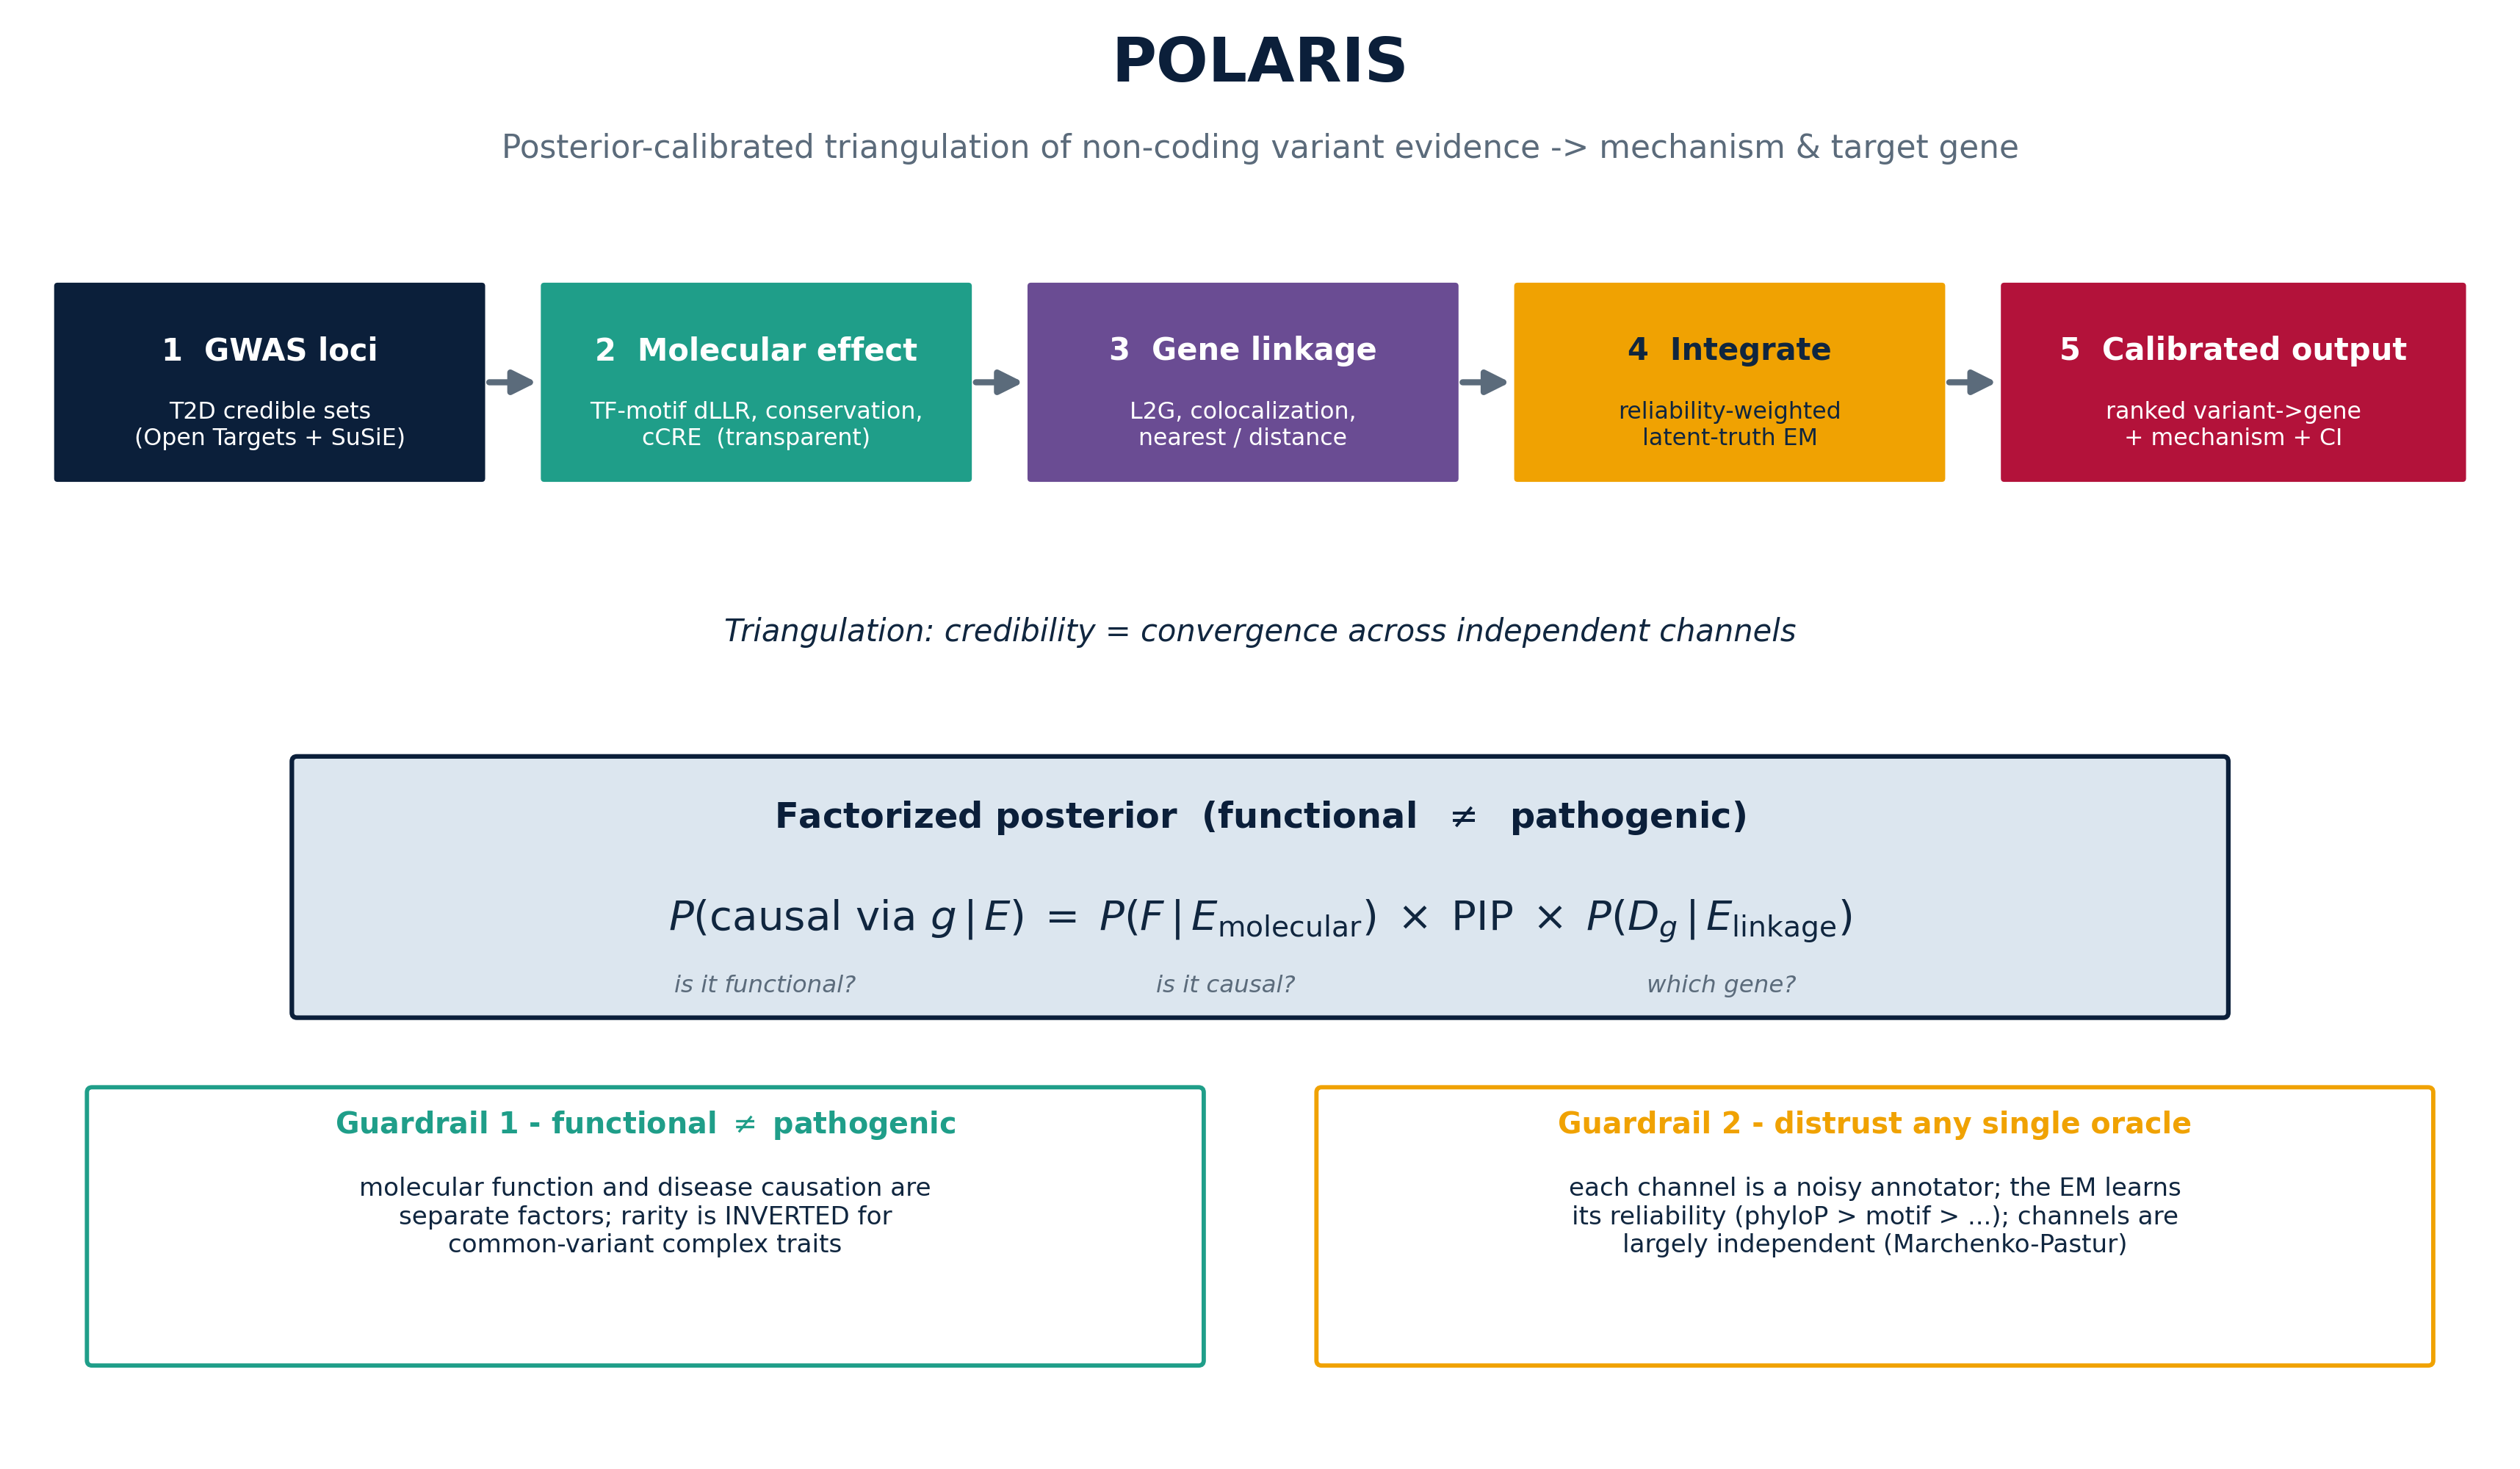
\includegraphics[width=0.84\linewidth]{fig_pipeline.png}
\caption{The whole pipeline at a glance, and the factorized posterior that separates ``functional'' from
``pathogenic.''}\label{fig:pipe}\end{figure}
\begin{figure}[h]\centering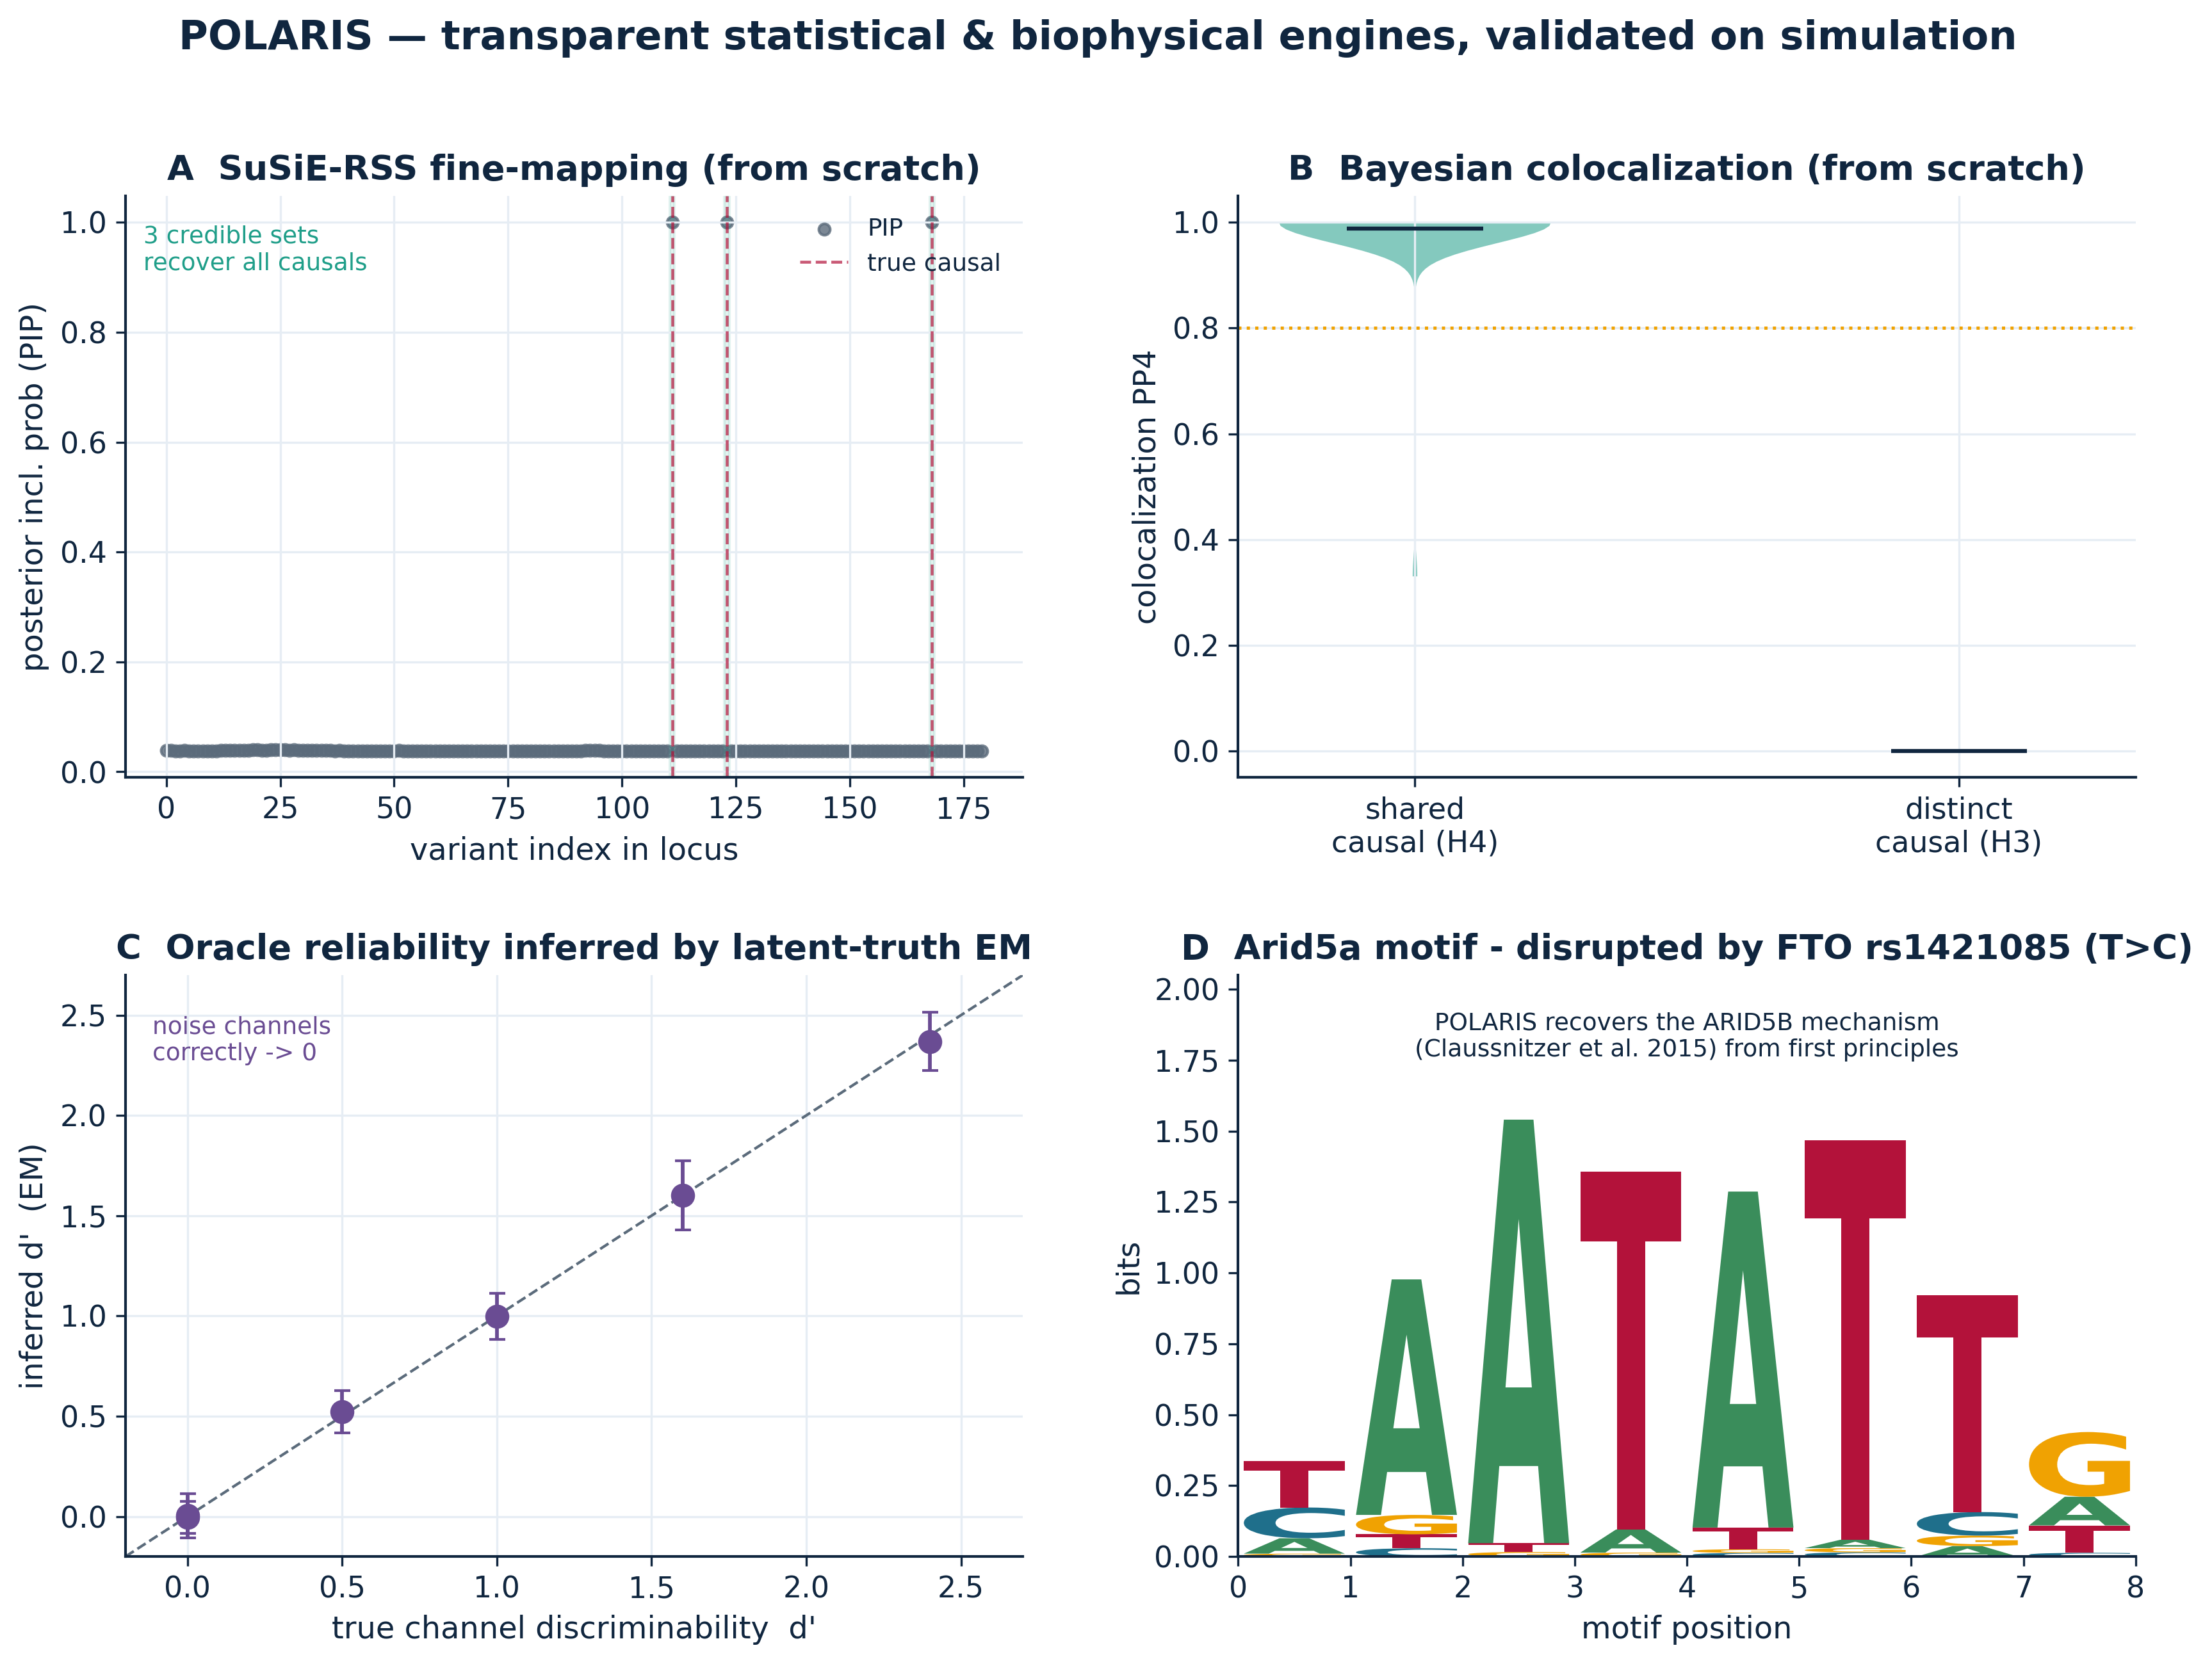
\includegraphics[width=0.84\linewidth]{fig_methods_validation.png}
\caption{Every engine was built from scratch and checked on data where we know the right answer.}\label{fig:methods}\end{figure}
\begin{figure}[h]\centering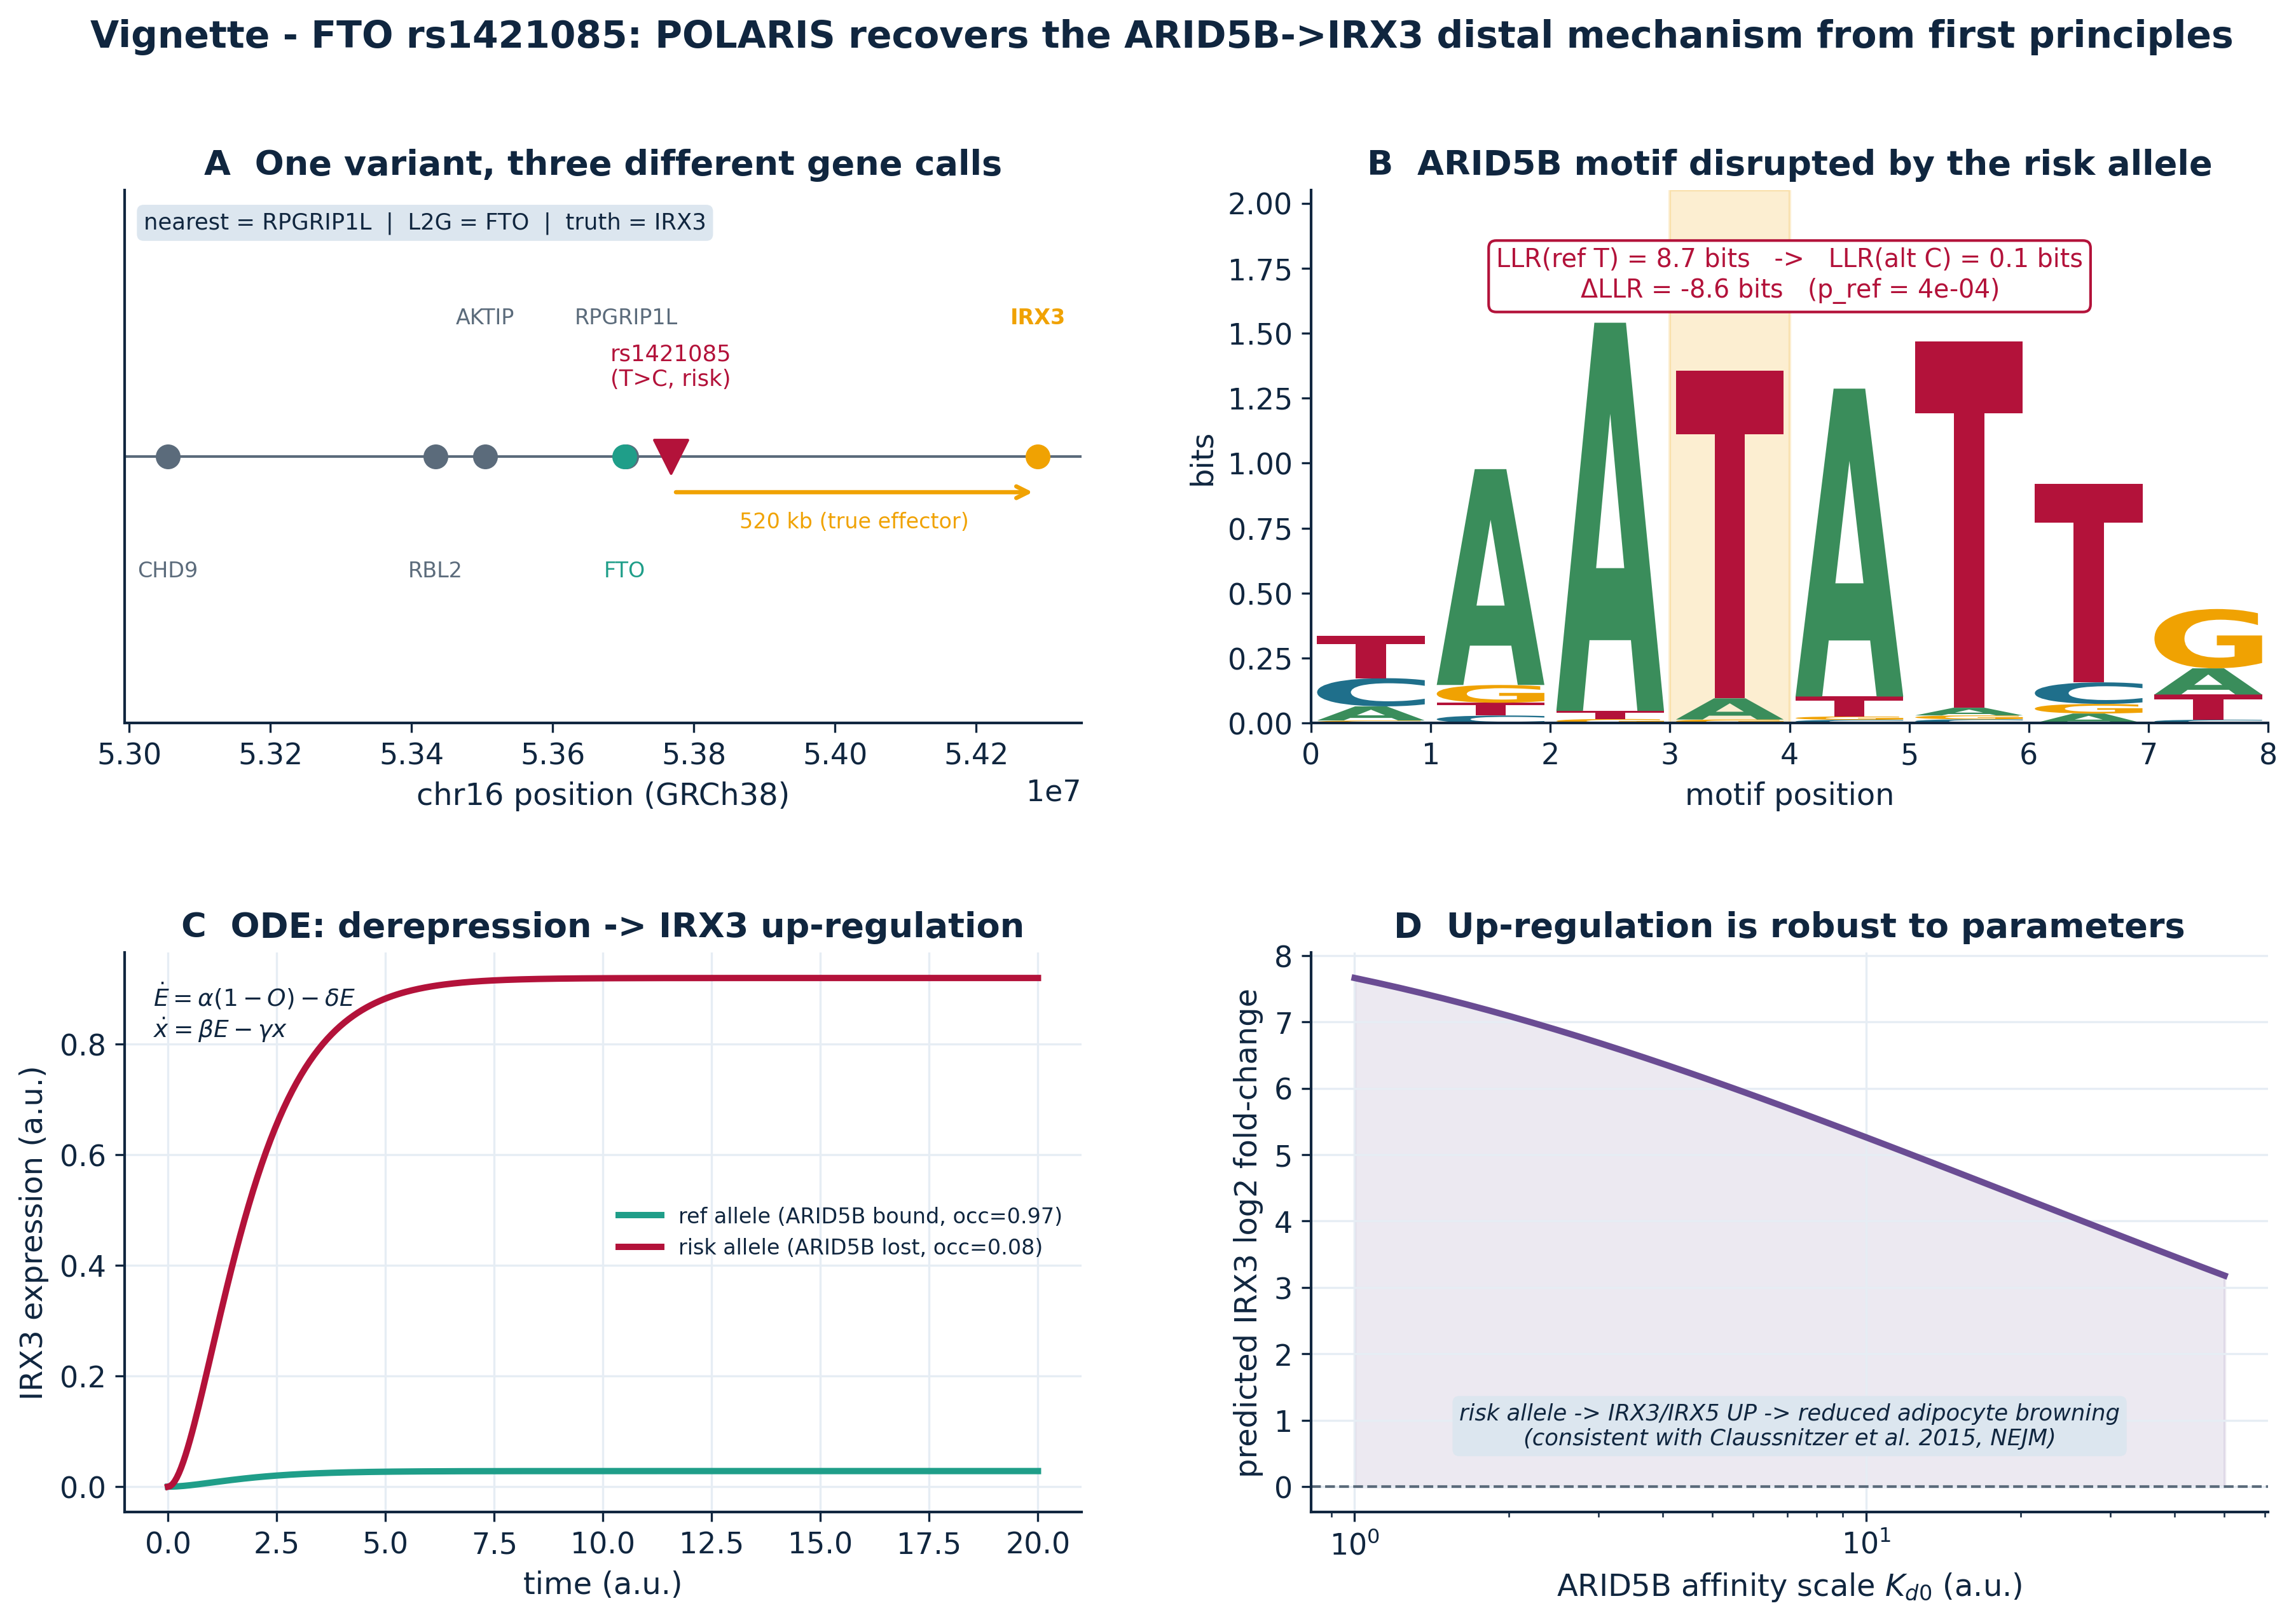
\includegraphics[width=0.84\linewidth]{fig_vignette_fto.png}
\caption{The \emph{FTO} story, end to end: locus confusion, the broken ARID5B grip site, and the
differential-equation prediction.}\label{fig:vignette}\end{figure}
\begin{figure}[h]\centering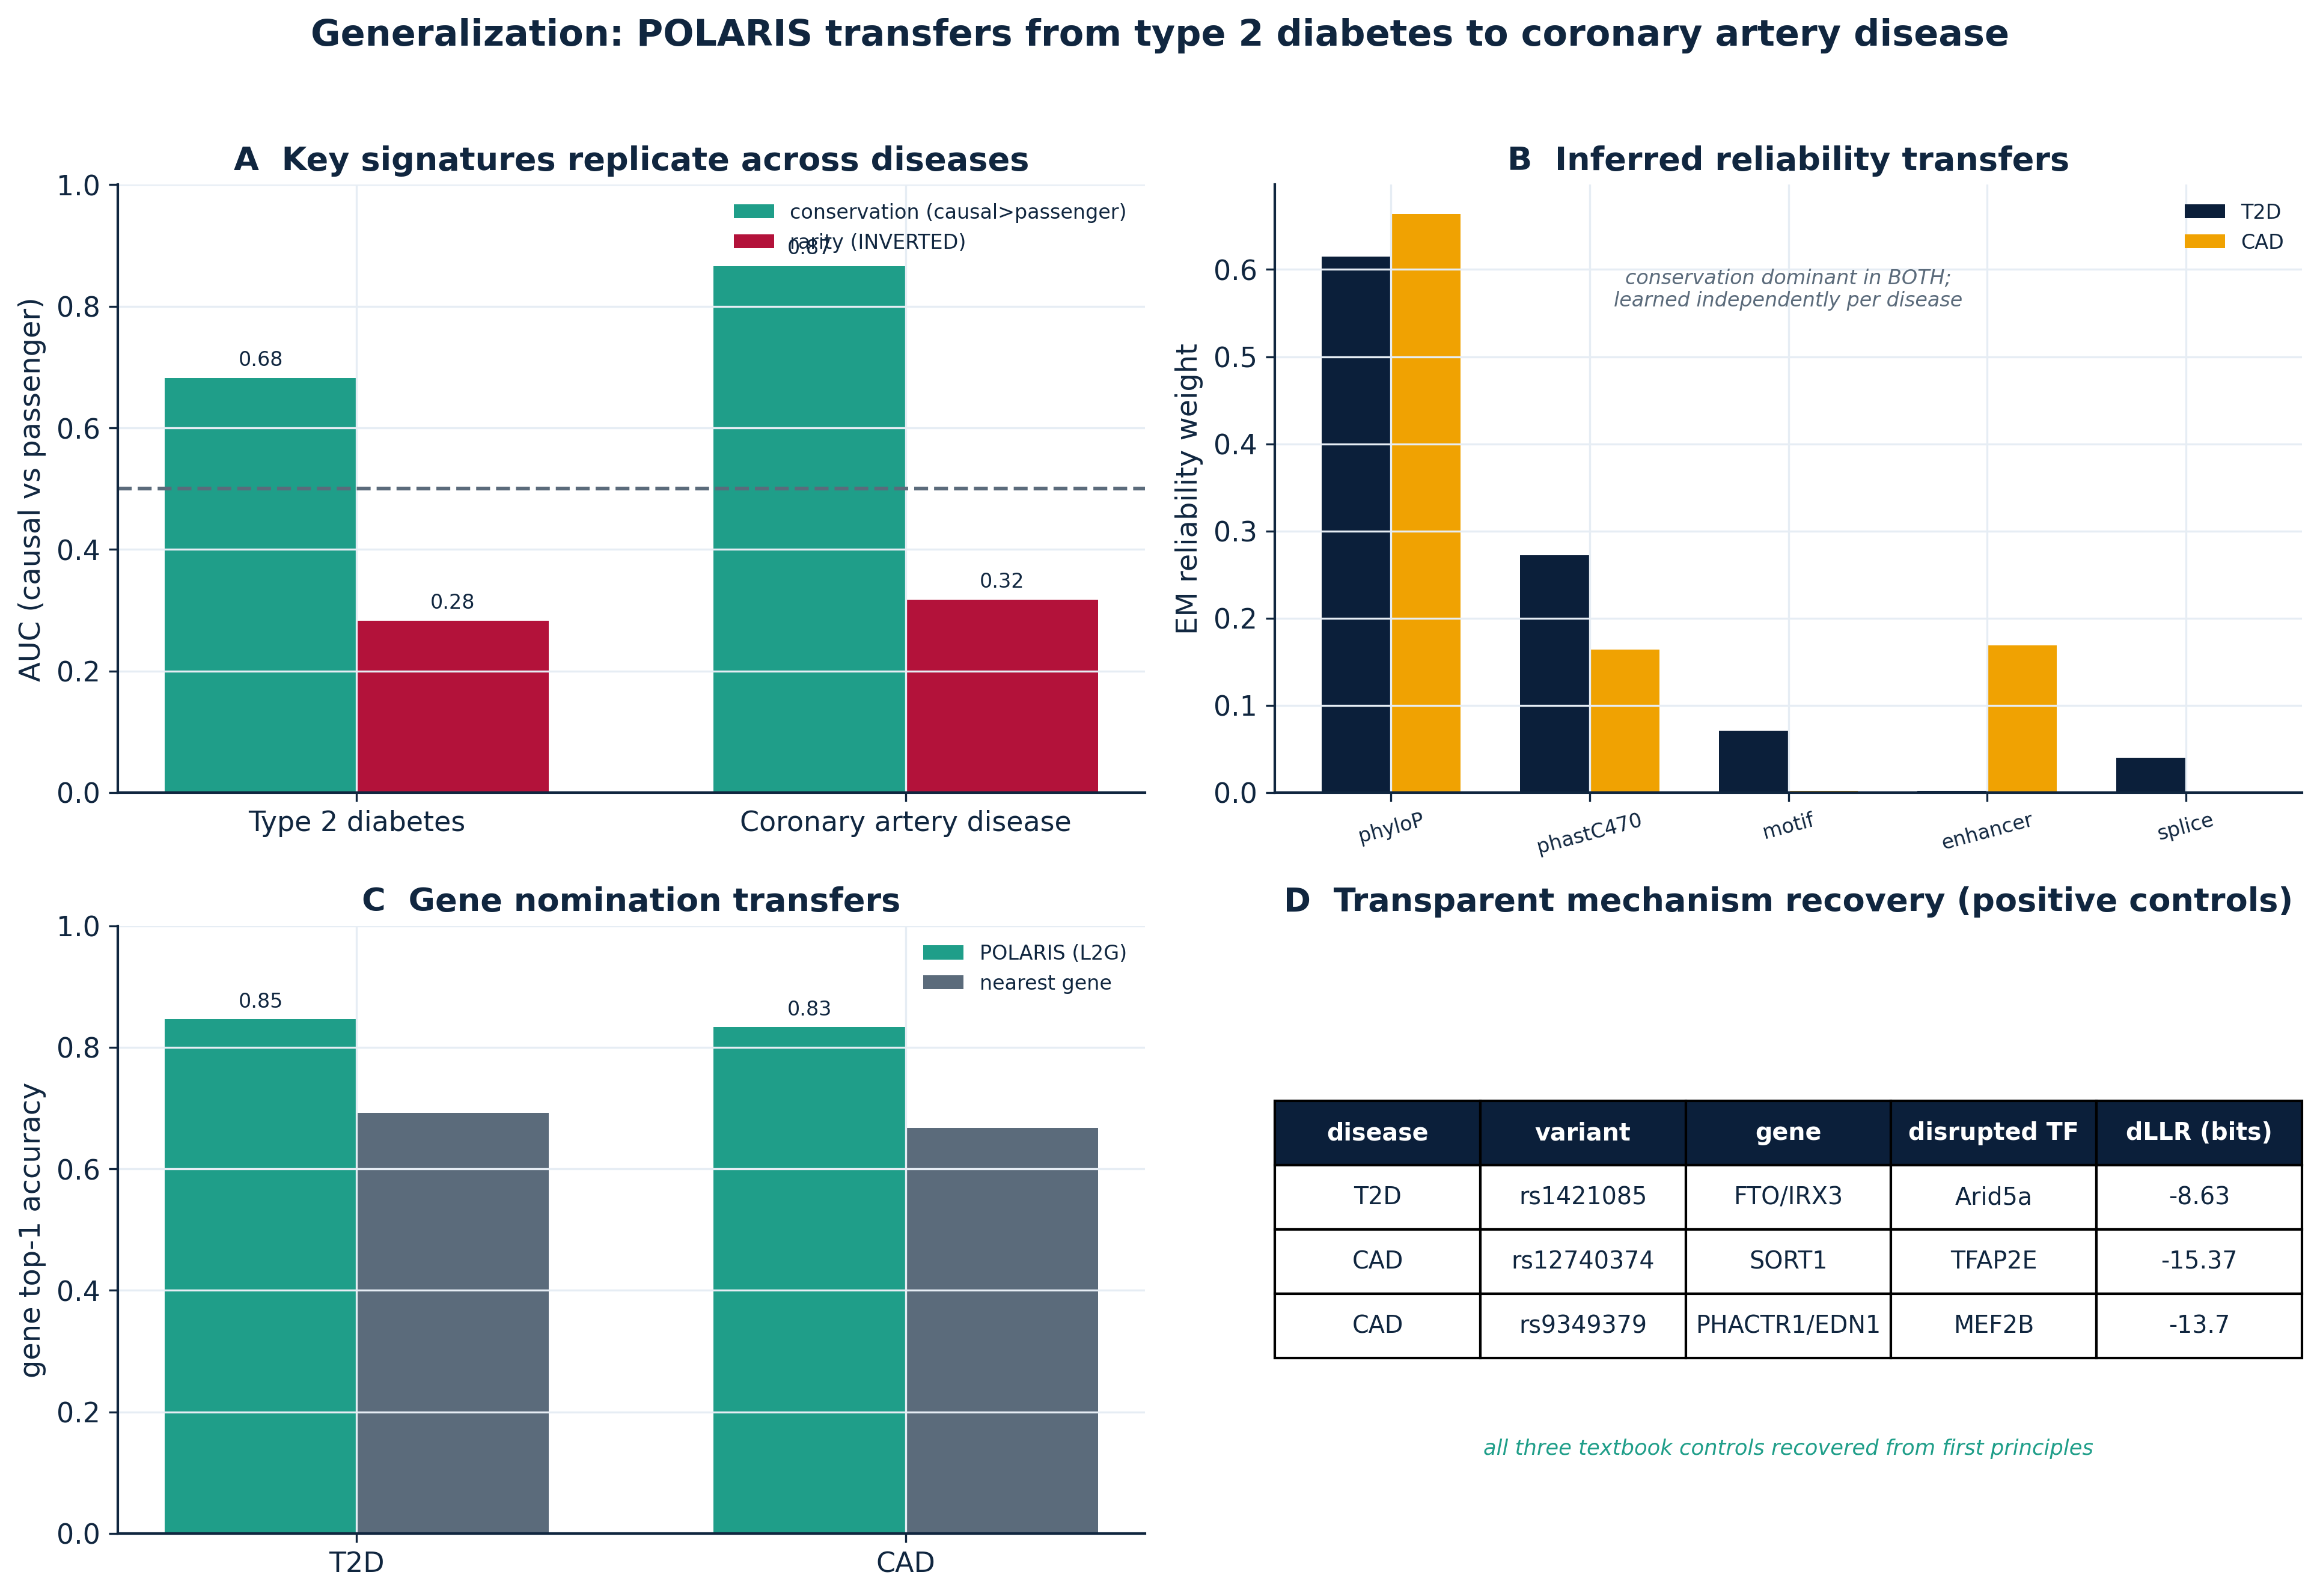
\includegraphics[width=0.84\linewidth]{fig_generalization.png}
\caption{The same behavior transfers to a second disease --- evidence it is a real method, not a fluke.}\label{fig:gen}\end{figure}

\end{document}
